% Created 2013-09-08 Sun 11:46
\documentclass[11pt]{article}
\usepackage[utf8]{inputenc}
\usepackage[T1]{fontenc}
\usepackage{fixltx2e}
\usepackage{graphicx}
\usepackage{longtable}
\usepackage{float}
\usepackage{wrapfig}
\usepackage[normalem]{ulem}
\usepackage{textcomp}
\usepackage{marvosym}
\usepackage{wasysym}
\usepackage{latexsym}
\usepackage{amssymb}
\usepackage{amstext}
\usepackage{hyperref}
\tolerance=1000
\usepackage{tikz}
\usepackage{tikz}
\usepackage{tikz-cd}
\usetikzlibrary{matrix,arrows,positioning,scopes,chains}
\tikzset{node distance=2cm, auto}
\author{Brian Beckman}
\date{\today}
\title{Fluent, Composable Error Handling}
\hypersetup{
  pdfkeywords={},
  pdfsubject={},
  pdfcreator={Emacs 24.3.1 (Org mode 8.0.7)}}
\begin{document}

\maketitle
\tableofcontents


\section{Introduction}
\label{sec-1}

Consider a program composed of \emph{serially dependent computations},
any of which produces either a value to feed to the next computation
in-line, or an error. If any computation in the sequence produces an
error, no downstream computations should be attempted and that error
should be the result of the entire sequence.

We show a sequence of solutions of increasing elegance in Java and
Clojure for this program. The solutions are in fluent style, which
minimizes the number of temporary variables that must be invented
and named. This style directly mimics the abstract data flow of the
solution.

We further show techniques for fluent error handling, both with
exceptions and with returned error codes.
\section{Motivating Example Problem}
\label{sec-2}

As a concrete example, suppose we must
get an authorization token, do a database lookup, do a web-service
call, filter the results of that call, do another web-servie call,
and then combine the results. The data flow of our program
resembles that in figure \ref{fig:dataflow}.

\begin{figure}
\begin{center}
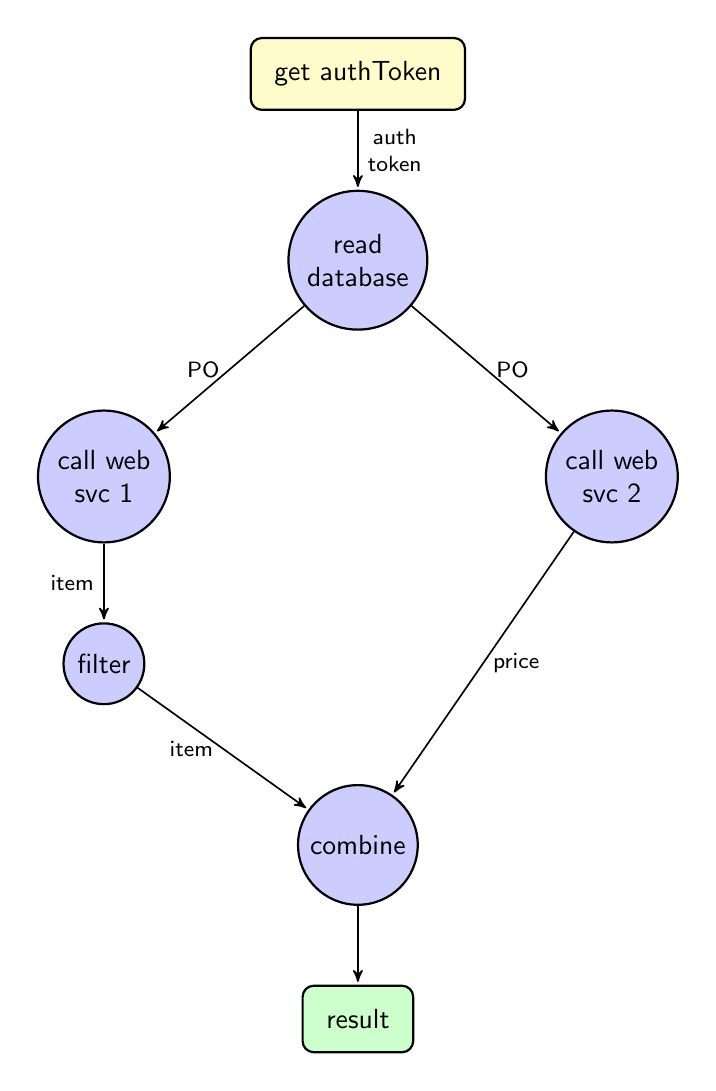
\begin{tikzpicture}[
  font=\sffamily,
  every matrix/.style={ampersand replacement=\&,column sep=1cm,row sep=1cm},
  source/.style={draw,thick,rounded corners,fill=yellow!20,inner sep=.3cm},
  process/.style={draw,thick,circle,fill=blue!20},
  sink/.style={source,fill=green!20},
  rectangle/.style={draw,very thick,shape=rectangle,inner sep=.3cm},
  dots/.style={gray,scale=2},
  invisible/.style={},
  to/.style={->,>=stealth',shorten >=1pt,semithick,font=\sffamily\footnotesize},
  every node/.style={align=center}]

  % Position  nodes using a matrix layout
  \matrix{
      {}
      \& \node[source] (auth) {get authToken};
      \& \\

      {}
      \& \node[process] (database) {read\\database};
      \& \\

      \node[process] (wscall1) {call web\\svc 1};
      \& 
      \& \node[process] (wscall2) {call web\\svc 2}; \\

      \node[process] (filter) {filter};
      \&
      \& \node[invisible] (placeholder) {}; \\

      {}
      \& \node[process] (combine) {combine};
      \& \\

      {}
      \& \node[sink] (result) {result};
      \& \\
  };

  % Draw the arrows between the nodes and label them.
  \draw[to] (auth) -- node[midway,right] {auth\\token} (database);
  \draw[to] (database) -- node[midway,left] {PO} (wscall1);
  \draw[to] (database) -- node[midway,right] {PO} (wscall2);
  \draw[to] (wscall1)  -- node[midway,left] {item} (filter);
  \draw[to] (filter)   -- node[midway,left] {item} (combine);
  \draw[to] (wscall2)  -- node[midway,right] {price} (combine);
  \draw[to] (combine)  -- (result);

\end{tikzpicture}
\end{center}
\caption{\label{fig:dataflow}Serially dependent computations}
\end{figure}

\subsection{Fluent Solution in Java, No Error Handling}
\label{sec-2-1}

In the \mbox{C++ -- like} languages, including JavaScript and Java,
we might keep intermediate results in instance variables and model
the flow as methods that produce instances from instances, that is,
as \textbf{transforms}. This style is called \textbf{fluent style}
because the text of the program resembles the flow in the diagram.

Imagine a \emph{main} program like the following, in which transforms are
on their own lines, indented from their \emph{sources} by one
\mbox{4-space} tab stop. The \textbf{source} of a transform is an
expression that produces an object.

\begin{verbatim}
public static void main(String[] args) {
    Computation databaseResults = new Computation()
        .authorize()
        .readDatabase();
    String result = databaseResults
        .callWebService()
        .filterResults()
        .combineResults(databaseResults
            .callOtherWebService());
    System.out.println(result); } }
\end{verbatim}

Notice that we save the \emph{Computation} produced by reading the
database in its own local variable, namely \emph{databaseResults}. We do
so because the dataflow branches from that result and we need to
use it twice, once as the source for calling the first web service
and once as the source for calling the second web service. If not
for this branching and recombining of the dataflow, we might have
written the entire program as one, fluent expression. 

The following is a complete program that mocks out the database and
web-service calls and can be compiled and executed, even online in
some service like \url{http://www.compileonline.com/compile_java_online.php}.

\begin{verbatim}
public class Computation {
    private String authToken;
    private String databaseResults;
    private String webServiceCallResults;
    private String filteredWebServiceCallResults;
    private String otherWebServiceCallResults;

    public Computation () {}
    public Computation authorize() {
        authToken = "John's credentials";
        return this; }
    public Computation readDatabase() {
        databaseResults = "{\"name\":\"John\", \"PO\":\"421357\"}";
        return this; }
    public Computation callWebService() {
        webServiceCallResults =
            "{\"item\":\"camera\", \"item\":\"shoes\"}";
        return this; }
    public Computation filterResults() {
        filteredWebServiceCallResults =
            "{\"item\":\"camera\"}";
        return this; }
    public Computation callOtherWebService() {
        otherWebServiceCallResults = "{\"price\":\"420.00\"}";
        return this; }
    public String combineResults(Computation other) {
        return "{[" + filteredWebServiceCallResults +
            "," + otherWebServiceCallResults + "]}"; }

    public static void main(String[] args) {
        Computation databaseResults = new Computation()
            .authorize()
            .readDatabase();
        String result = databaseResults
            .callWebService()
            .filterResults()
            .combineResults(databaseResults
                .callOtherWebService());
        System.out.println(result); } }
\end{verbatim}
\subsection{Fluent Solution in Java, with Exceptions}
\label{sec-2-2}

The program above has \emph{no} error handling. One of the better ways
techniques for error handling in fluent style is with exceptions.
If each sub-computation is responsible for throwing its own
exception with error details, then a single try-catch suffices to
get error details out of the overall sequence, leaving the
essential dataflow expression unchanged. Our main routine has
minimal changes, and becomes simply

\begin{verbatim}
public static void main(String[] args) {
    try {
        Computation databaseResults = new Computation()
            .authorize()
            .readDatabase();
        String result = databaseResults
            .callWebService()
            .filterResults()
            .combineResults(databaseResults
                .callOtherWebService());
        System.out.println(result); }
    catch (Exception e) {
        System.out.println(e.getMessage());
}   }
\end{verbatim}
noting, in passing, that resource freeing (database connections,
sockets, file handles, etc.) is ignored here.\footnote{Idiomatically,
   resource management can be handled in a \emph{finally} clause or with
   Java 7's automatic resource management. See \url{http://bit.ly/15GYkMh}}

Let's give each mocked sub-computation a \mbox{10\%} chance of
erroring, and our entire sample becomes just the following:

\begin{verbatim}
import java.util.Random;
public class Computation {
    private String authToken;
    private String databaseResults;
    private String webServiceCallResults;
    private String filteredWebServiceCallResults;
    private String otherWebServiceCallResults;
    private static Random random = new java.util.Random();
    private static Boolean randomlyError() {
        return random.nextDouble() < 0.10; }

    public Computation () {}
    public Computation authorize() throws Exception {
        if (randomlyError()) { throw new Exception("auth errored"); }
        authToken = "John's credentials";
        return this; }
    public Computation readDatabase() throws Exception {
        if (randomlyError()) { throw new Exception("database errored"); }
        databaseResults = "{\"name\":\"John\", \"PO\":\"421357\"}";
        return this; }
    public Computation callWebService() throws Exception {
        if (randomlyError()) { throw new Exception("ws1 errored"); }
        webServiceCallResults =
            "{\"item\":\"camera\", \"item\":\"shoes\"}";
        return this; }
    public Computation filterResults() throws Exception {
        if (randomlyError()) { throw new Exception("filter errored"); }
        filteredWebServiceCallResults =
            "{\"item\":\"camera\"}";
        return this; }
    public Computation callOtherWebService() throws Exception {
        if (randomlyError()) { throw new Exception("ws2 errored"); }
        otherWebServiceCallResults = "{\"price\":\"420.00\"}";
        return this; }
    public String combineResults(Computation other) throws Exception {
        if (randomlyError()) { throw new Exception("combine errored"); }
        return "{[" + filteredWebServiceCallResults +
            "," + otherWebServiceCallResults + "]}"; }

    public static void main(String[] args) {
        try {
            Computation databaseResults = new Computation()
                .authorize()
                .readDatabase();
            String result = databaseResults
                .callWebService()
                .filterResults()
                .combineResults(databaseResults
                    .callOtherWebService());
            System.out.println(result); }
        catch (Exception e) {
            System.out.println(e.getMessage());
}   }   }
\end{verbatim}
\subsection{Fluency Lost Without Exceptions}
\label{sec-2-3}

Error handling with exceptions is
debatable,\footnote{\url{http://www.joelonsoftware.com/items/2003/10/13.html}}
especially in Java where runtime exceptions need not be
declared,\footnote{\url{http://bit.ly/1e5P6Cg}} but the alternative of checked
exceptions can be considered harmful.\footnote{\url{http://bit.ly/9NyrdD}}

Rather than join the debate, just imagine that we have decided
against exceptions for whatever reason and see if we can write
reasonable code.

Add a private String field, \emph{errorResult}, and let every method set
the error result if and only if it errors. We must change
\emph{combineResults}; it can no longer return just a \emph{String}, but
rather a \emph{Computation}, because it may, itself, produce an error.
Furthermore, we lose the fluent style because every call must be
individually checked.

A particularly nasty way to do this is as follows:

\begin{verbatim}
public static String computation () {
    Computation c1 = new Computation();
    Computation c2 = c1.authorize();
    if (c2.errorResult.isEmpty()) {
        Computation c3 = c2.readDatabase();
        if (c3.errorResult.isEmpty()) {
            Computation c4 = c3.callWebService();
            if (c4.errorResult.isEmpty()) {
                Computation c5 = c4.filterResults();
                if (c5.errorResult.isEmpty()) {
                    Computation c6 = c3.callOtherWebService();
                    if (c6.errorResult.isEmpty()) {
                        Computation c7 = c5.combineResults(c6);
                        if (c7.errorResult.isEmpty()) {
                            return c7.getResult(); }
                        else {return c7.errorResult;} }
                    else {return c6.errorResult;} }
                else {return c5.errorResult;} }
            else {return c4.errorResult;} }
        else {return c3.errorResult;} }
    else {return c2.errorResult;} }
public static void main(String[] args) {
    System.out.println(computation()); }
\end{verbatim}

This is so intolerable as to barely deserve criticism, despite the
fact that its working set is optimized for the positive
path!\footnote{The error branches are all at addresses far from the
   non-error branches, which are clustered together for  maximum locality.} We've
lost any correspondence between the program text and the program
specification, and all options for nesting and placement of curly
braces are ludicrous.

The prevailing style, nowadays, is to reverse all the branches and
to return as early as possible from the main routine. Despite the
fact that multiple returns were condemned in the
dogma of structured programming and are lethal in code that
manages resources,\footnote{\url{http://bit.ly/sAvDmY}} the
justification for this is two-fold:
\begin{itemize}
\item it results in linear code that can be read from top to bottom
\item modern compilers can reverse the branches in the generated code
automatically after a post-compilation profiling
step\footnote{\url{http://en.wikipedia.org/wiki/Profile-guided_optimization}}
\end{itemize}

This alternative\footnote{favored in the previously cited
   Joel-on-Software blog} is the following:

\begin{verbatim}
public static String computation() {
    Computation c1 = new Computation();
    Computation c2 = c1.authorize();
    if (! c2.errorResult.isEmpty()) {return c2.errorResult;}
    Computation c3 = c2.readDatabase();
    if (! c3.errorResult.isEmpty()) {return c3.errorResult;}
    Computation c4 = c3.callWebService();
    if (! c4.errorResult.isEmpty()) {return c4.errorResult;}
    Computation c5 = c4.filterResults();
    if (! c5.errorResult.isEmpty()) {return c5.errorResult;}
    Computation c6 = c3.callOtherWebService();
    if (! c6.errorResult.isEmpty()) {return c6.errorResult;}
    Computation c7 = c5.combineResults(c6);
    if (! c7.errorResult.isEmpty()) {return c7.errorResult;}
    return c7.getResult(); }
public static void main(String[] args) {
    System.out.println(computation()); }
\end{verbatim}

This, at least, gets rid of the ludicrous nesting, but exposes another
deep weakness: we have a proliferation of temporary variables just to
hold the \emph{Computations} returned by the intermediate stages. Why
bother with this when we have no hope of fluent style? Let's go to

\begin{verbatim}
public static String computation() {
    Computation c1 = new Computation();
    c1.authorize();
    if (! c1.errorResult.isEmpty()) {return c1.errorResult;}
    c1.readDatabase();
    if (! c1.errorResult.isEmpty()) {return c1.errorResult;}
    c1.callWebService();
    if (! c1.errorResult.isEmpty()) {return c1.errorResult;}
    c1.filterResults();
    if (! c1.errorResult.isEmpty()) {return c1.errorResult;}
    c1.callOtherWebService();
    if (! c1.errorResult.isEmpty()) {return c1.errorResult;}
    c1.combineResults(c1);
    if (! c1.errorResult.isEmpty()) {return c1.errorResult;}
    return c1.getResult(); }
public static void main(String[] args) {
    System.out.println(computation()); }
\end{verbatim}

The whole program, now, is the following

\begin{verbatim}
import java.util.Random;
public class Computation {
    private String errorResult;
    private String result;
    private String authToken;
    private String databaseResults;
    private String webServiceCallResults;
    private String filteredWebServiceCallResults;
    private String otherWebServiceCallResults;
    private static Random random = new java.util.Random();
    private static Boolean randomlyError() {
        return random.nextDouble() < 0.10; }

    public Computation () {errorResult=""; result="no result";}
    public Computation authorize() {
        if (randomlyError()) { errorResult = "auth errored"; }
        authToken = "John's credentials";
        return this; }
    public Computation readDatabase() {
        if (randomlyError()) { errorResult = "database errored"; }
        databaseResults = "{\"name\":\"John\", \"PO\":\"421357\"}";
        return this; }
    public Computation callWebService() {
        if (randomlyError()) { errorResult = "ws1 errored"; }
        webServiceCallResults =
            "{\"item\":\"camera\", \"item\":\"shoes\"}";
        return this; }
    public Computation filterResults() {
        if (randomlyError()) { errorResult = "filter errored"; }
        filteredWebServiceCallResults =
            "{\"item\":\"camera\"}";
        return this; }
    public Computation callOtherWebService() {
        if (randomlyError()) { errorResult = "ws2 errored"; }
        otherWebServiceCallResults = "{\"price\":\"420.00\"}";
        return this; }
    public Computation combineResults(Computation other) {
        if (randomlyError()) { errorResult = "combine errored"; }
        result = "{[" + filteredWebServiceCallResults +
            "," + otherWebServiceCallResults + "]}"; 
        return this;}
    public String getResult() {return result;}
    public static String computation() {
        Computation c1 = new Computation();
        c1.authorize();
        if (! c1.errorResult.isEmpty()) {return c1.errorResult;}
        c1.readDatabase();
        if (! c1.errorResult.isEmpty()) {return c1.errorResult;}
        c1.callWebService();
        if (! c1.errorResult.isEmpty()) {return c1.errorResult;}
        c1.filterResults();
        if (! c1.errorResult.isEmpty()) {return c1.errorResult;}
        c1.callOtherWebService();
        if (! c1.errorResult.isEmpty()) {return c1.errorResult;}
        c1.combineResults(c1);
        if (! c1.errorResult.isEmpty()) {return c1.errorResult;}
        return c1.getResult(); }
    public static void main(String[] args) {
        System.out.println(computation());
}   }
\end{verbatim}
\section{Let's Do Better}
\label{sec-3}

So packaged, we may write the program
directly as a sequence \emph{via} Clojure's \verb|->| or \verb|->>| or
the \verb|let| syntax, as follows:

\begin{verbatim}
(try
  (let [auth-token        (get-auth-token)
        db-results        (read-database auth-token)
        svc-results       (call-web-service db-results)
        other-svc-results (call-other-web-service svc-results)
        filtered-results  (filter my-predicate 
      read-database

  (catch Exception e (.getMessage e)))
\end{verbatim}

The desired behavior is similar to that of the Maybe
monad,\footnote{\url{http://en.wikipedia.org/wiki/Monad_(functional_programming)}\#The$_{\text{Maybe}}$$_{\text{monad}}$}
the difference being that \emph{Maybe} just produce \emph{Nothing} if anything
goes wrong. The consumer of the computation doesn't know what stage
of the pipeline failed nor any details at all about the error.
\emph{Maybe} suppresses all that. Such a situation is not tolerable in
the real world. Consider the example of a database retrieval
followed by a few web-service calls followed by a filter and
transformation followed by a logging call followed by output to UI
components. If something goes wrong in this sequence of
computations, we need to know exactly where and as much detail as
we can get about the failure. But we certainly don't want any
computations downstream of the failure to be attempted.

\section{Code}
\label{sec-4}

\begin{figure}[H]
\label{project-file}
\begin{verbatim}
(defproject ex1 "0.1.0-SNAPSHOT"
  :description "Project Fortune's Excel Processor"
  :url "http://example.com/TODO"
  :license {:name "TODO"
            :url "TODO"}
  :dependencies [[org.clojure/clojure     "1.5.1"]
                 [org.clojure/algo.monads "0.1.4"]
                 [org.clojure/data.zip    "0.1.1"]
                 [dk.ative/docjure        "1.6.0"]
                ]
  :repl-options {:init-ns ex1.core})
\end{verbatim}
\end{figure}

\begin{figure}[H]
\label{main-namespace}
\begin{verbatim}
(ns ex1.core
  (:use clojure.algo.monads))
\end{verbatim}
\end{figure}

\begin{figure}[H]
\label{main-monad}
\begin{verbatim}
(defmonad if-not-error-m
  [m-result (fn [value] value)
   m-bind   (fn [value f]
              (if-not (:error value)
                (f value) 
                value))
   m-zero   {:error "unspecified error"}
   m-plus   (fn [& mvs]
              (first (drop-while :error mvs)))

   ])
\end{verbatim}
\end{figure}

\begin{figure}[H]
\label{main-test-namespace}
\begin{verbatim}
(ns ex1.core-test
  (:require [clojure.test        :refer :all]
            [ex1.core            :refer :all]
            [clojure.algo.monads :refer :all]))
\end{verbatim}
\end{figure}

\begin{figure}[H]
\label{test-monads}
\begin{verbatim}
(deftest exception-throwing-test
  (testing "exceptions are thrown"
    (is (thrown? ArithmeticException (/ 1 0)))
    (is (thrown-with-msg? ArithmeticException #"Divide by zero" (/ 1 0)))
    ))

(deftest comprehension-test
  (testing "sequence monad and comprehension"
    (is (= (domonad sequence-m
                    [a (range 5)
                     b (range a)]
                    (* a b))
           (for [a (range 5)
                 b (range a)]
             (* a b)))
        "Monadic sequence equals for comprehension")))

(defn- divisible? [n k]
  (= 0 (rem n k)))

(def ^:private not-divisible?
  (complement divisible?))

(defn- divide-out [n k]
  (if (divisible? n k)
    (recur (quot n k) k)
    n))

(defn- error-returning-check-divisibility-by [k n]
  (let [q (divide-out n k)]
    (if (= q n)
      {:error (str n ": not divisible by " k)}
      q)))

(defn- exception-throwing-check-divisibility-by [k n]
  (let [q (divide-out n k)]
    (if (= q n)
      (throw (Exception.
              (str {:error (str n ": not divisible by " k)})))
      q)))

(defn- best-small-divisor-sample [a2]
  (try
    (->> a2
        (exception-throwing-check-divisibility-by 2)
        (exception-throwing-check-divisibility-by 3)
        (exception-throwing-check-divisibility-by 5)
        (exception-throwing-check-divisibility-by 7))
    (catch Exception e (.getMessage e)))
  )

()

(defn- ugly-small-divisor-sample [a2]
  (if (not-divisible? a2 2)
    {:error (str a2 ": not divisible by 2")}
    (let [a3 (quot a2 2)]
      (if (not-divisible? a3 3)
        {:error (str a3 ": not divisible by 3")}
        (let [a5 (quot a3 3)]
          (if (not-divisible? a5 5)
            {:error (str a5 ": not divisible by 5")}
            (let [a7 (quot a5 5)]
              (if (not-divisible? a7 7)
                {:error (str a7 ": not divisible by 7")}
                {:success (str a7 ": divisible by 2, 3, 5, and 7")}
                )
              )
            )
          )
        )
      )
    )
  )

(defn- not-pretty-enough-small-divisor-sample [a2]
  (with-monad if-not-error-m
    (->
     (m-bind (m-result a2 ) (fn [a2]  (m-result (error-returning-check-divisibility-by 2 a2))))
     (m-bind  (fn [a3]  (m-result (error-returning-check-divisibility-by 3 a3))))
     (m-bind  (fn [a5]  (m-result (error-returning-check-divisibility-by 5 a5))))
     (m-bind  (fn [a7]  (m-result (error-returning-check-divisibility-by 7 a7))))
     )))

(defn- prettier-small-divisor-sample [a2]
  (domonad if-not-error-m
           [a3  (error-returning-check-divisibility-by 2 a2)
            a5  (error-returning-check-divisibility-by 3 a3)
            a7  (error-returning-check-divisibility-by 5 a5)
            a11 (error-returning-check-divisibility-by 7 a7)
            ]
           a11))

(defn- even-prettier-small-divisor-sample [a2]
  (with-monad if-not-error-m
    ((m-chain
      [(partial error-returning-check-divisibility-by 2)
       (partial error-returning-check-divisibility-by 3)
       (partial error-returning-check-divisibility-by 5)
       (partial error-returning-check-divisibility-by 7)
       ])
     a2)))

(defn- prettiest-small-divisor-sample [a2]
  (with-monad if-not-error-m
    ((m-chain
      (vec (map #(partial error-returning-check-divisibility-by %)
                [2 3 5 7])))
     a2)))

(deftest if-not-error-monad-test
  (testing "the if-not-error-monad"
    (is (=
         (ugly-small-divisor-sample 42)
         (prettier-small-divisor-sample 42)))
    (is (=
         (ugly-small-divisor-sample 42)
         (not-pretty-enough-small-divisor-sample 42)))
    (is (=
         (ugly-small-divisor-sample 42)
         (even-prettier-small-divisor-sample 42)))
    (is (=
         (ugly-small-divisor-sample 42)
         (prettiest-small-divisor-sample 42)))    )
)
\end{verbatim}
\end{figure}
\section{References}
\label{sec-5}

\section{Conclusion}
\label{sec-6}
% Emacs 24.3.1 (Org mode 8.0.7)
\end{document}
